\documentclass{article}

\usepackage{lmodern}
\usepackage[T1]{fontenc}
\usepackage[utf8]{inputenc}

% Drafting

\usepackage[latexmk]{lwarp}

\usepackage{xcolor,soul}
\usepackage{fullpage}
\usepackage{setspace}
\usepackage{blindtext}
\doublespacing

\definecolor{mwcolor}{HTML}{8af67d}
\definecolor{vgcolor}{HTML}{c88bff} % MPL purple
\definecolor{citecolor}{HTML}{c696f0} % MPL purple


% Tools for leaving todo notes around
\usepackage[colorinlistoftodos]{todonotes}
%% \renewcommand{\todo}{}
%% \renewcommand{\hl}[1]{#1}
\newcommand{\citeme}[1]{%
  \todo[color=citecolor]{%
  \ifstrempty{#1}{[citation needed]}{[cite: #1]}%
  }%
}
\newcommand{\mw}[2]{%
  \sethlcolor{mwcolor}\hl{#2}\sethlcolor{yellow}%
  \ifstrempty{#1}{}{%
    \todo[color=mwcolor]{#1 [MW]}%
  }%                  
}
\newcommand{\vg}[2]{%
  \sethlcolor{vgcolor}\hl{#2}\sethlcolor{yellow}%
  \ifstrempty{#1}{}{%
    \todo[color=vgcolor]{#1 [VG]}%
  }%                  
}


\usepackage{graphicx}
\usepackage[version=4]{mhchem}
\usepackage{siunitx}
\usepackage[hidelinks]{hyperref}
\usepackage{glossaries}
\usepackage{xr} % For cross-referencing wit the supplemental information
\usepackage{textgreek}

\newcommand{\nca}[1]{\ce{Li_{#1}Ni_{0.8}Co_{0.15}Al_{0.05}O_2}}
\DeclareRobustCommand{\nmc}[2][]{%
    \ifstrempty{#1}{%
        \ce{Li_{#2}Ni_{y}Mn_{z}Co_{1-y-z}O2}}{}%
    \ifstrequal{#1}{333}{%
        \ce{Li_{#2}Ni_{1/3}Mn_{1/3}Co_{1/3}O2}}{}%
    \ifstrequal{#1}{532}{%
        \ce{Li_{#2}Ni_{0.5}Mn_{0.3}Co_{0.2}O2}}{}%
}

% Techniques
\newacronym{xrd}{PXRD}{powder X-ray diffraction}
\newacronym{uxrd}{µ-XRD}{X-ray microdiffraction}
\newacronym{txm}{TXM}{transmission X-ray microscopy}
\newacronym{xas}{XAS}{X-ray absorbance spectroscopy}
\newacronym{xanes}{XANES}{X-ray absorbance near edge spectroscopy}
\newacronym{iscat}{iSCAT}{optical interferometric scattering microscopy}

% Facilities and organizations
\newacronym{ssrl}{SSRL}{Stanford Synchrotron Radiation Lightsource}

% Chemistry
%\newacronym{ecd}{ECD}{exchange current density}
\newacronym{ecd}{$i_0$}{exchange current density}
\newacronym{od}{OD}{optical depth}
\newacronym{ocv}{OCV}{open circuit voltage}

% Particles in u-XRD mapping
\newacronym{p1}{P1}{particle 1}
\newacronym{p2}{P2}{particle 2}
\newacronym{p3}{P3}{particle 3}


\usepackage{authblk}

\title{Origin of Rapid Delithiation In Secondary Particles Of \nca{} and \nmc{} Cathodes}

\author[1,2,3]{Mark Wolfman}
\author[1]{Brian M.\ May}
\author[4]{Vishwas Goel}
\author[4]{Sicen Du}
\author[5,6]{Young-Sang Yu}
\author[7]{Nicholas V.\ Faenza}
\author[7]{Nathalie Pereira}
\author[8]{Antonin Grenier}
\author[3]{Kamila M.\ Wiaderek}
\author[3]{Ruqing Xu}
\author[9]{Jiajun Wang}
\author[8]{Karena W.\ Chapman}
\author[7]{Glenn G. Amatucci}
\author[4]{Katsuyo Thornton}
\author[1]{Jordi Cabana\thanks{Corresponding author: jcabana@uic.edu}}

\affil[1]{Department of Chemistry, University of Illinois at Chicago}
\affil[2]{Chemical Sciences and Engineering Division, Argonne National Laboratory}
\affil[3]{X-ray Science Division, Advanced Photon Source, Argonne National Laboratory}
\affil[4]{Department of Materials Science and Engineering, University of Michigan}
\affil[5]{Department of Physics, Chungbuk National University}
\affil[6]{Advanced Light Source, Lawrence Berkeley National Laboratory}
\affil[7]{Energy Storage Research Group, Department of Materials Science and Engineering, Rutgers, The State University of New Jersey}
\affil[8]{Department of Chemistry, Stony Brook University}
\affil[9]{Harbin Institute of Technology}

\date{}


\newlength{\figwidth}
\setlength{\figwidth}{3.5in}

\myexternaldocument{supplement}

\begin{document}

\maketitle

\begin{abstract}
  Most research on the electrochemical dynamics in battery materials
  has focused on the global behavior of the electrode. There has been
  debate within recent literature on the origin of an apparent
  two-phase transformation within layered cathodes for Li-ion
  batteries. The work presented here uses nano-focused X-ray probes to
  measure delithiation \textit{in operando} at the scale of secondary
  particle agglomerates in \nca{} and \nmc{} cathodes during
  charge. After an initial latent phase, individual secondary
  particles undergo rapid, stochastic, and largely uniform
  delithiation, which is in contrast with the gradual increase in
  potential measured for the whole cell. These results provide direct
  evidence that the apparent two-phase transition is emergent from
  kinetic limitations governing a population of secondary
  particles. Physics modeling further links this behavior to an
  increase in \gls{ecd} over three orders of magnitude within a narrow
  range of delithiation. The specifics and implications of this jump
  in \gls{ecd} are crucial to understanding the charge-storage
  reaction of Li-ion battery cathodes.
\end{abstract}

\listoftodos

%%%%%%%%%%%%%%%%%%%%%%%
\section{Introduction}
%%%%%%%%%%%%%%%%%%%%%%%

\begin{itemize}
\item \citeme{wang2020-6} -> Feng's TXM/XANES NMC-811 paper
\item \citeme{chueh2021} -> Will Chueh's in-situ XRD/STXM NMC-333 paper
\item \citeme{rao2021} -> iSCAT of LCO particles during cycling: saw
  individual particles going and maybe linked it to diffusion? (check
  that last part)
\end{itemize}

% NCA/NMC material
Layered transition metal oxides represent the state-of-the-art of
cathodes materials for electrochemical energy storage. In order to
meet ever more ambitious performance targets, it will be necessary to
improve their efficiency and reliability beyond current
limitations. While layered cathodes provide high theoretical capacity,
only \SI{\approx70}{\percent} is realistically achievable, with a
steeper penalty imposed at higher rates\citeme{}. This observation
points to kinetic barriers preventing full utilization of the
cathode. Careful observation of local heterogeneity, combined with
detailed simulation of the underlying electrochemical processes, can
reveal details of the kinetic factors governing these reactions,
ultimately leading to higher performing energy storage systems. 

% TXM/XRD background

Synchrotron X-ray characterization provides several methods to
evaluate heterogeneity within secondary particles of layered cathode
materials. \Gls{uxrd} extends the structural characterization of
conventional \gls{xrd} with improved spatial resolution. Incoming
X-rays are focused to a sub-micron spot and scanned over individual
secondary particles. At each mapping position, the diffraction pattern
captured by an area detector provides details of the crystal
structure, such as the unit-cell parameters, which can then be related
to chemical states (e.g.\ extent of lithiation). A complementary
technique, \Gls{txm}, produces projection micrographs showing the
optical depth of the object with \SI{\approx30}{nm} spatial
resolution, depending on the instrument configuration. The tunable
nature of synchrotron X-ray sources allows micrographs of the same
field of view to be captured at several energies. To produce chemical
maps, images are collected at a range of energies spanning an X-ray
absorption edge, producing a separate spectrum for each pixel in the
field of view and, after data reduction, a chemical map with chemical
significance (e.g.\ metal oxidation states). For both techniques,
since the individual measurements are projections through the
specimen, the resulting maps show the average state through the
optical axis (perpendicular to the image plane).

The high transmission provided by hard X-rays is conducive to making
measurements inside an assembled cell (is-situ) and, ideally, while
the cell is actively cycling (operando). In addition to avoiding
relaxation effects, in-situ measurement allows the same object to be
measured repeatedly at different states of charge. Tracking the same
object during a (dis)charge cycle allows for a direct comparison
between different states of charge and provides a clearer picture of
how heterogeneity evolves.

%% NCA/NMC background

Ensemble \gls{xrd} has shown a mixture of phases in \nca{} electrodes
during the first charge when stored in ambient conditions, in contrast
with the solid-solution, single-phase transformation seen during
subsequent charge cycles\cite{robert2015}. A possible origin is the
presence of a lithium diffusion barrier arising from surface
\ce{Li2CO3} formation upon exposure to \ce{CO2} and \ce{H2O}. When
pristine \nca{} was protected from ambient air exposure, a
single-phase solid-solution reaction was observed during first
charge\cite{grenier2017}. This observation led to the conclusion that
the secondary particles contained an uneven coating of \ce{Li2CO3},
which must be broken electrochemically before the reaction can
proceed. The need to break this coating would produce different
timelines for reaction initiation in different particles, resulting in
a bimodal distribution of oxidation states and the appearance of
non-equilibrium heterogeneity by \gls{xrd}.

The oxidation states of individual secondary particles were measured
by operando \gls{txm} \gls{xas} and, indeed, particles were observed
to be either in a pristine or partially oxidized state with more
particles becoming oxidized at higher states of
charge\cite{nowack2016}. While \ce{Li2CO3} clearly plays a role in the
ability of lithium to penetrate into the secondary particle, it was
also demonstrated that the presence of two phases by \gls{xrd} is
suppressed by stronger compaction of the electrode during laminate
preparation\cite{bobrikov2018}. A related layered cathode material,
\nmc[333]{}, is less prone to \ce{Li2CO3} formation, even showing
lower levels of \ce{Li2CO3} after one month of air exposure than those
found in pristine \nca{}\cite{shizuka2007}. In-situ \gls{xrd} studies
of \nmc[333]{} during first charge show a largely single-phase
(solid-solution) transformation \cite{hulzen2018,ahn2017,zhou2016-2},
though some studies reveal two crystallographic phases with a small
difference in \emph{a} and \emph{c} unit-cell parameters and
coexisting over a narrow range of delithiation compared to
\nca{}\cite{yoon2006,hua2018}. The oxidation dynamics of these layered
cathode materials warrant further study to clarify the nature of the
chemical transformation, especially in view of locating the onset and
progression of heterogeneity, within and between the secondary
particles that typically compose a cathode. It is important to
elucidate how general this behavior is among the general class of
layered oxides that are leading candidates as battery materials.

This work further examined the heterogeneities present in secondary
particles of established layered cathode materials, namely \nca{},
\nmc[333]{}, and \nmc[532]{}. A combination of operando \gls{uxrd} and
\gls{txm} \gls{xas} experiments probed both the inter-particle
heterogeneity. While the cell potential and prior reports of ensemble
\gls{xas} indicated a smooth transition to higher oxidation state upon
delithiation\cite{deb2005,muto2009}, individual particles exhibited a
sharp and stochastic transition from an initial, latent state to one
containing highly oxidized \ce{Ni}. Physics simulations were then
conducted to determine the role of fundamental electrochemical
processes in generating this rapid delithiation behavior, determined
to result from a rapid rise in the exchange current density covering
several orders of magnitude over a narrow range of lithium
compositions.

%%%%%%%%%%%%%%%%%%%%%%%%%%%%%%%%%%%%%%%%%%%%%%%%%
\section{Operando Characterization}
%%%%%%%%%%%%%%%%%%%%%%%%%%%%%%%%%%%%%%%%%%%%%%%%%

%% \subsection{\Gls{uxrd} - Interparticle Dynamics}

Lithiation of several secondary particles of \nca{} was tracked during
first change and discharge using operando \gls{uxrd} mapping. For each
particle, the individual area diffraction patterns collected at each
X--Y mapping position were integrated to one-dimensional patterns, and
subsequently summed for all points collected during the reaction
(Figures \ref{fig:uxrd}a,b and \ref{fig:xrd-echem}). The diffraction
patterns for all three particles in the pristine condition were
consistent with those previously reported for \nca{}
\cite{novak2015}. There was an extra feature that varied in
intensity at Q\SI{\approx3.6}{\per\angstrom}, representative of
metallic \ce{Li} (PDF \#00-001-1131). Small extraneous peaks occurred
due to random aberrations in individual pixels on the diffraction
detector (Figure \ref{fig:xrd-echem}).

The diffraction peaks for \gls{p1} began to shift in $Q$ soon after
the onset of oxidation (Figure \ref{fig:uxrd}a). The shifts observed
in \gls{p1} were consistent with similar observations of
\emph{operando} \gls{xrd} of the ensemble average\cite{robert2015},
as opposed to individual particles in \nca{} electrodes, in prior
work\cite{grenier2017}. \gls{p2} (\ref{fig:xrd-echem}b) also
exhibited changes in peak positions during cycling. While the peak
positions of the extreme states (pristine, charged, discharged) were
consistent with those of \gls{p1}, the peaks did not begin shifting
until the cell had reached a higher potential
\SI{\approx4.5}{\volt}. During discharge, peaks in both \gls{p1} and
\gls{p2} shifted to lower $Q$ at approximately the same rate. \gls{p3}
(\ref{fig:xrd-echem}c) showed no apparent changes in diffraction peak
positions during charge or discharge, possibly due to poor electrical
connection to the carbon and binder of the electrode.

Consideration of individual peaks provided more detailed structural
information. The (003) reflection showed an initial decrease in $Q$
(Figure \ref{fig:uxrd}a), representing an expansion of the $c$ axis
due to stacking of the alternating transition metal and lithium
layers\citeme{}. The initial decrease in $Q$ was followed by a sudden
increase in $Q$ beyond the initial state, indicating contraction of
the lattice along the $c$ axis during delithiation. This trend has
been reported before. The initial expansion is attributed to
electrostatic repulsion between \ce{O^{2-}} ions in neighboring layers
once the shielding effect of deintercalated \ce{Li+} ions is no longer
present\cite{robert2015}. In turn, the subsequent collapse is driven
by steric effects, and reflects the near complete removal of \ce{Li+}
ions, which previously acted as pillars in the layered
framework. Simultaneously, the (104) diffraction peak gradually
shifted to higher $Q$ (lower $d$) upon removal of \ce{Li} from the
material (Figure \ref{fig:uxrd}b). This shift reflected the balance
between the trend along $c$ and the continuous decrease in the $a$
dimension. In this case, the decrease was attributed to the shortening
of metal--oxygen distances due to the oxidation of the transition
metal ions (mainly \ce{Ni}), resulting in smaller ionic radii.

Unit cell parameters for each particle were refined from diffraction
patterns using the Le Bail method, and plotted as a function of cell
potential for \gls{p1} and \gls{p2} (Figures \ref{fig:uxrd}d and
\ref{fig:cell-pars}). The refined unit cell parameters matched the
qualitative trends described above in Figures \ref{fig:uxrd}a,b and
\ref{fig:xrd-echem}, as well as measurements of the ensemble average
of an electrode available in the literature\cite{novak2015}. The
cell parameters for \gls{p1} began shifting at a cell potential
somewhere between \SIrange{3.0}{3.8}{\volt} (Figure
\ref{fig:uxrd}d). The precise value is unknown since the temporal
resolution of the experiment was insufficient to capture a full map
during the rapid increase in potential at the beginning of charge. The
unit cell parameters for \gls{p2} began shifting at
\SI{\approx4.5}{\volt} (\ref{fig:cell-pars}c,d), consistent with the
peak shifts in \ref{fig:xrd-echem}b. These results led to the
qualitative conclusion that the rates of delithiation of each
individual particle were different and not uniquely represented by the
electrochemical response collected for the whole electrode.

%% \subsection{u-XRD - Rates of (De)lithiation}

The rate of delithiation can be quantified by estimating the amount of
\ce{Li} present in the material at different points during cathode
oxidation based on unit-cell parameters reported for ensemble-average
\gls{xrd} in Robert \emph{et al}\cite{robert2015}. In this reference
study, \nca{} was cycled twice with a cutoff potential of
\SI{4.8}{\volt} and the cell parameters were associated with the
average \ce{Li} content in the material based on coulometric
calculations. During the first cycle, the overall \nca{} electrode
underwent a heterogeneous transformation driven by kinetic limitations
due to the presence of \ce{Li2CO3}, which is electronically
insulating, on the particle surfaces. \ce{Li2CO3} is oxidized to
\ce{CO2} during this first charge. As a result, in the second cycle,
the electrode transformed via the expected solid-solution pathway. We
compared our data to the second cycle from the work by Robert et al.,
since we did not see any evidence of heterogeneity in either the
electrochemistry or diffraction of individual particles
(\ref{fig:xrd-echem}). In order to directly compare trends in \ce{Li}
content, the experimental unit cell parameters were adjusted to ensure
agreement between the pristine state presented here first value for
the second charge of the reference data presented by Roberts et al.,
accounting for scalar discrepancies in the measurement.

Figure \ref{fig:uxrd}e shows the \ce{Li} content in \nca{x} as a
function of time during the first charge-discharge cycle, based on the
measured change in \emph{c} parameter. Similar trends were observed
when calculating \ce{Li} content using the \emph{a} parameter (Figure
\ref{fig:rates}). To allow for easier comparison between experiments
and simulation, lithiation was shown as a ratio of time passed to the
total time to reach the cutoff potential ($t_c$). This measure is
sensitive to experimental conditions, such as the choice of cut-off
potential, and so absolute comparisons are only valid within an
experiment. For both \gls{p1} and \gls{p2} the rate of delithiation
was initially slow, followed by a sudden increase (Figure
\ref{fig:uxrd}e). In the case of \gls{p1}, the delithiation during the
first \SI{0.05}{t_c} proceeded at \SI{\approx0.025}{\ce{Li}\per\hour},
or C/40, followed by a deceleration until \SI{0.2}{t_c} passed. After
this period, the overall content of the particle was
\ce{Li_{0.88}Ni_{0.80}Co_{0.15}Al_{0.05}O2}. At this point, the
reaction dramatically accelerated nearly 10-fold from the initial
rate, to \SI{\approx0.3}{\ce{Li}\per\hour}, or C/3.33 until an average
composition \nca{0.53} where the rate decelerated again until the sign
of the current was reverted. In the case of \gls{p2} there was very
little delithiation for the first \SI{0.8}{t_c}. Delithiation
proceeded down to an average content of \nca{0.92} at
\SI{\approx0.03}{\ce{Li}\per\hour}, or C/33, followed by a 20-fold
increase in rate, to \SI{\approx0.66}{\ce{Li}\per\hour}, or
C/1.5. When an average composition \nca{0.53} was again reached, the
reaction slowed down, running below \SI{0.1}{\ce{Li}\per\hour}, or
C/10, for the remainder of the oxidation. Particles relithiated
rapidly during cell discharge, with no periods of slow activity. The
states that were captured showed faster rates of relithiation earlier
in the discharge for both \gls{p1} and \gls{p2}, rivaling the fastest
rates at intermediate contents of \ce{Li} in \nca{x}, qualitatively
consistent with the oxidation. \todo{I don't understand this last
  sentence}

%% \subsection{XRD Discussion}

\gls{p1} and \gls{p2} both achieved the same level of delithiation at
the end of the charge sequence, observed in Figure \ref{fig:uxrd}e and
by the peak positions in Figures \ref{fig:uxrd}a,b and
\ref{fig:ind-peaks}. Since \gls{p2} did not start delithiating until
late in the charge sequence, its maximum rate of delithiation was more
than double that of \gls{p1}. This observation has no precedent in the
literature for reactions involving solid solutions, where homogeneity
removes the activation barrier toward nucleation of two-phase
mechanisms. It is particularly intriguing considering that the whole
electrode was discharged at a low constant current. It can be
hypothesized that it is due to subtle variations in overpotential
between particles as a result of a different connectivity with the
electrical circuit through the carbon additive (electrons) and the
pores that contain electrolyte (ions). Particle size may have also had
an impact. Since \gls{p2} was approximately half the size of \gls{p1},
the \ce{Li} diffusion lengths out of the particle would have been
shorter. Neither of these explanations is satisfactory to predict the
change in rate for an individual particle. It is worth noting that the
changes happen at approximately similar \ce{Li} contents for both
particles studied, suggesting that the oxidation of the material
changes its physical properties, such as electronic and ionic
conductivity. Follow-up experiments are needed to evaluate this
point. Both particles relithiated to \nca{x}, where $x$ was between
\numrange{0.88}{0.97}.

%% \subsection{TXM - \nmc{}}

%% \subsubsection{\nmc[333]{} Inter-particle Dynamics}

\Gls{txm} \gls{xas} was also used to characterize \nca{} secondary
particles during charge, providing a direct, spatially resolved probe
of \ce{Ni} oxidation states. Dilute (\SI{20}{\percent}) \nca{}
electrodes were assembled in modified coin-cells, and operando
\gls{txm} \gls{xas} frame-sets were collected during the first
galvanostatic charge/discharge cycle (Figure
\ref{fig:txm-nca}). Localized \gls{xas} K-edge spectra were produced
from operando \gls{txm} frame-sets and then averaged over all pixels
in secondary particle agglomerates. A \gls{txm} frame showing several
particles in a field of view is shown in Figure \ref{fig:txm-nca}a. Upon
delithiation, a progressive increase was seen in the energy of the
absorption edge and the associated whiteline (Figures
\ref{fig:isobestic-point} and \ref{fig:kedges}). Ideally, chemically
pure reference samples are prepared for the two chemical end-members,
and the observed spectra analyzed by linear combination fitting of the
two reference spectra, as is done for
\ce{LiFePO4}\cite{wanli2016}. However, the absence of a miscibility
gap for layered cathodes prevents the preparation of chemically pure
reference samples. Instead, a more direct approach is used. For
layered transition-metal oxide cathodes, the energy of maximum
absorbance, or whiteline, of the \ce{Ni} K-edge increases as
\ce{Ni^{3+}} oxidizes to \ce{Ni^{4+}}. Therefore, whiteline energy was
used as a proxy for \ce{Ni} oxidation, which is the dominant redox
process in \nca{}.

Fields of view containing multiple secondary particles were selected
from within the coin-cell window (Figure \ref{fig:txm-nca}a), allowing
comparison of the dynamics between separate particles. Additionally,
several cells were prepared at select states of delithiation and
measured by ex-situ ensemble \gls{xas} (Figure
\ref{fig:txm-nca}c). This allowed a comparison between whiteline
position and average state-of-charge for each particle as a function
of time (Figure \ref{fig:txm-nca}d). Initially, the whiteline energies
were constant, indicating no \ce{Ni} oxidation. After
\SIrange{0.4}{0.6}{t_c}, the whiteline energies increased rapidly,
reaching \SIrange{75}{100}{\percent} state-of-charge. Although some
particles oxidized simultaneously with one another, there was no clear
preference for when particles began rapid oxidation. Not all of the
particles measured reached the full \SI{100}{\percent}
state-of-charge. Additionally, upon reaching their maximum
state-of-charge, some particles subsequently exhibited \ce{Ni}
reduction, presumably due to oxygen loss resulting in conversion to a
cubic rock-salt-like phase\citeme{}. This stochastic particle-level
behavior was in contrast with the that seen by in-situ
ensemble-average \gls{xas}\cite{deb2005}, which showed a gradual
increase in whiteline position over the full range of
delithiation. Overall, this inter-particle rapid oxidation was in
agreement with the observations made by \gls{uxrd} described above
(Figure \ref{fig:uxrd}).

\begin{table}
  \begin{tabular}{c c c | c c c}
    \multicolumn{3}{c|}{\nmc[333]{x}} & \multicolumn{3}{c}{\nca{x}} \\
    x & Whiteline /eV & \textDelta{} /eV & x & Whiteline /eV & \textDelta{} /eV \\
    \hline\hline
    0.945 & 8353.98 & 0.21 & 1.00 & 8348.84 & 0.00 \\
    0.751 & 8354.72 & 0.94 & 0.80 & 8349.61 & 0.78 \\
    0.570 & 8355.45 & 1.68 & 0.60 & 8350.14 & 1.30 \\
    0.386 & 8356.12 & 2.35 & 0.25 & 8350.78 & 1.95 \\
    0.257 & 8356.43 & 2.66 & 0.00 & 8351.16 & 2.32 \\
  \end{tabular}
  \caption{Reported energies of \ce{Ni} K-edge whiteline. In-situ
    \gls{xas} of \nmc[333]{} (Ref.\ \cite{deb2005}) and ex-situ
    \gls{xas} \nca{} (Ref.\ \cite{muto2009}). Data extracted from
    published figures using
    WebPlotDigitizer\cite{webplotdigitizer}. Relative shifts in
    whiteline energy (\textDelta{}) calculated as difference from
    fully lithiated state (x=1).}
  \label{tab:bulk-xas-extraction}
\end{table}

%% \subsubsection{\nmc[532]{}}

To evaluate the similarity in the oxidation behavior of \nca{} to
other layered cathode compositions, similar \gls{txm} \gls{xas}
experiments were performed on cells containing dilute \nmc[333]{} and
\nmc[532]{} layered cathodes (Figure \ref{fig:txm-nmc}). Compared to
\nca{} (Figure \ref{fig:txm-nca}a), \nmc{} particle were less
spherical in shape (Figure \ref{fig:txm-nmc}a). Since no
ensemble-average measurements were performed, the mean optical depth
for all foreground pixels in the frame was used for evaluating overall
oxidation (Figures \ref{fig:txm-nmc}b,c). Similarly to \nca{}, spectra
for both \nmc{} cathodes showed an increase in the whiteline
energy. \nmc[333]{} exhibited a lower initial whiteline energy. The
\ce{Mn{3+}/Mn{4+}} redox couple has a higher reduction potential than
the \ce{Ni{2+}/Ni{3+}} couple, which results in the spontaneous
formation of \ce{Ni^{2+}} limited by the concentration of manganese
(lower in the case of \nmc[532]{}). Rather than calculate an average
state-of-charge, as was done when ensemble-average spectra were
available (as presented for \nca{} above, Figure \ref{fig:txm-nca}d),
whiteline energies were compared to the lowest value observed for any
particle in the field of view during the operando experiment, reported
here as \textDelta{}whiteline. A parametric function was fit to each
pixel's full spectrum, and the whiteline energies were extracted from
the fit parameters. This approach provided higher precision and was
more tolerant of noise between frames, allowing for faster time
resolution. For both \nmc{} materials, the same initial latent phase
and subsequent rapid oxidation were seen (Figures
\ref{fig:txm-nmc}d,e). The initial rapid \ce{Ni} oxidation resulted in
changes in whiteline energy for \nmc[333]{} of
\SI{\approx3}{\electronvolt} and \nmc[532]{} of
\SI{\approx2.5}{\electronvolt}, reflecting the lower starting
concentration of \ce{Ni^{2+}} in \nmc[532]{}. The experiment using
\nmc[532]{} did not reach the same overall state of charge. For
\nmc[333]{}, once rapid oxidation had occurred, a subsequent gradual
increase to \SI{4.1}{eV} was observed for \nmc[333]{}. The total
change in whiteline energy for all observed secondary particles was
\SI{>4}{eV} (Figure \ref{fig:txm-nmc}d). While ensemble \gls{xas}
studies\cite{deb2005,muto2009} did not reach the \SI{4.7}{V} cell
cut-off potential needed for full lithium extraction and hence full
\ce{Ni} oxidation, extrapolation of the trend in Table
\ref{tab:bulk-xas-extraction} and Figure
\ref{fig:bulk-xas-extraction}a predicts a change in whiteline energy
upon full delithiation of \SI{\approx3}{eV}. This discrepancy between
particle-level and ensemble average \ce{Ni} oxidation suggests that an
appreciable portion of the particles in the specimens measured by
ensemble \gls{xas} had not reached their fully oxidized states.

In summary, all layered cathode chemistries studied exhibited
punctuated rapid delithiation at the secondary particle level. This
behavior was observed when measurements were made with independent
mapping techniques (\gls{uxrd} and \gls{txm}) and with both low-energy
(\SI{\approx8}{\kilo\electronvolt}) and high-energy
(\SI{25}{\kilo\electronvolt}) X-rays, and with varying carbon content
in the electrode composite. The persistent of this phenomena across
observations suggest that this behavior is inherent to layered cathode
materials rather than an artifact of the technique, further supported
by previous reports\cite{chueh2021}\citeme{rao2021 and others?}. These
results do not by themselves provide an explanation for why rapid
delithiation occurs between secondary particles. Detailed models of
delithiation dynamics are needed to link the observed behavior to
fundamental electrochemical processes, which are presented in the next
section.

\section{Dynamics Simulations}

%% Electrochemical dynamics simulations to identify the origin of the
%% accelerated delithiation

To identify the origin of the experimentally observed sequential
accelerated delithiation of individual \nca{} particles during the
galvanostatic charging of the electrode, electrochemical dynamics
simulations were performed on an \nca{}/Li cell model with 8
particles, ranging from \SIrange{4}{11}{\micro\meter} in diameter.

Since the electrodes used in the experiments were highly porous, they
are unlikely to be limited by electrolyte transport. Furthermore,
rapidly accelerating delithiation was observed in electrodes with both
\SI{60}{\percent} (\gls{txm}) and \SI{20}{\percent} (\gls{uxrd})
levels of carbon additive, so electronic conduction limitations are
also not a good candidate for explaining the observed
behavior. Therefore, the accelerated delithiation is attributed to
either the exchange current density, $i_0$, at the
particle/electrolyte interface, or \ce{Li^{+}} diffusivity in \nca{},
$D_S$.

To further narrow down the underlying cause, sensitivity analyses were
performed for both $i_0$ and $D_S$ at different C-rates. The results
of these analyses at C/20 are summarized below, while the results at
other C-rates are provided in the \mw{ref to specific
  section}{Supporting Information}. More details about the model,
including the governing equations and the complete set of parameters
employed, can also be found in the \mw{ref to specific
  section}{Supplementary Information}.

%% sensitivity analysses with respect to i_0

In this section, we report the results of the sensitivity studies with
respect to different forms of $i_0$. \ce{Li^+} diffusivity was set to
$D_S>\SI{5e-15}{\meter\squared\per\second}$ (obtained from
\cite{amin2015}) for all simulations in this section to avoid
solid-state limitation in the simulated system.

%% Selection of i_0 function

Traditionally, $i_0$ has been presumed to be directly proportional to
$X_{\rm{Li}}^{0.5}\left(1-X_{\rm{Li}}\right)^{0.5}$, where
$X_{\rm{Li}}$ is the \ce{Li^+} site fraction in the active
material\cite{newman1994-2,newman1993,newman1996,newman1995-2}. This
functional form results from the theoretical consideration that
\ce{Li^+} exists in a solid solution state in the active
material. However, recent studies have shown that such a dependence is
not applicable for materials like \nca{}\cite{chueh2021} and
\nmc{}\cite{mukherjee2017,chiang2020,tsai2018}. For example, Park et
al.\cite{chueh2021}\ reported an exponential dependence of $i_0$ on
$X_{\rm{Li}}$\cite{chueh2021}. Other studies have shown that $i_0$ is
a monotonically decreasing function of
$X_{\rm{Li}}$\cite{mukherjee2017,chiang2020,tsai2018}. Thus, the
dependence of $i_0$ on $X_{\rm{Li}}$ is not precisely
known. Furthermore, the literature is missing similar analysis for
$X_{\rm{Li}} > 0.92$.

To work with the uncertain form of $i_0$, two sets of simulations were
run. In the first set of the simulations, the traditional form of
$i_0$ is used (Figure \ref{fig:i0_profiles}). In the second set of
simulations, a model form of $i_0$ is used (Figure
\ref{fig:i0_profiles}). The model form was chosen to have a smooth
step function of $X_{\rm{Li}}$, generated by a cubic spline.

The traditional form only has the max value of $i_0$,
$i_{0,\rm{max}}$, as a tunable parameter, whereas the model form uses
four parameters: $i_{0,\rm{min}}$, the minimum value of $i_0$;
$i_{0,\rm{max}}$; $X_{\rm{Li}}^{\star}$, the value of $X_{\rm{Li}}$
where the transition begins from $i_{0,\rm{min}}$ to $i_{0,\rm{max}}$;
and $\Delta X_{\rm{Li}}$, the width of the transition zone. The
presence of additional parameters enables the model function of $i_0$
to represent most of the aforementioned functions from the
literature. Since the values of $i_{0,\rm{max}}$ reported in the
literature\cite{tsai2018,dees2008} do not vary widely, an intermediate
value of $i_0 = \SI{1}{\ampere\per\meter\squared}$ was selected. A
comparison of the $i_0$ values used in the traditional and model
functions to those from the literature is provided in Figure
\ref{fig:i0_profiles}.

%% Effects of i_0 on the dilithiation dynamics
The evolution of the volume-averaged Li-site fraction,
$\left<X_{\rm{Li}}\right>$, for the first set of simulations, i.e.,
with the traditional form of $i_0$ at \SI{0.05}{\per\hour} is provided
in Figure \ref{fig:i0_basic}. In this case, none of the particles
exhibit the accelerated delithiation behavior, and all the particles
delithiate at the same rate.

For the second set of simulations, the evolution results are presented
individually for the sensitivity analyses with respect to
$i_{0,\rm{min}}$, $X_{Li}^{\star}$, and $\Delta X_{\rm{Li}}$. The
results corresponding to $i_{0,\rm{min}}$ are provided here and the
remaining results are provided in the \mw{ref to specific
  section}{Supporting Information}.

Four different values of $i_{0,\rm{min}}$ were chosen, ranging from
\SIrange{0.01}{0.001}{\ampere\per\meter\squared}, with other
parameters as $i_{0,\rm{max}} = \SI{1}{\ampere\per\meter\squared}$,
$X_{\rm{Li}}^{\star} = 0.9$, and $\Delta X_{\rm{Li}} = 0.05$. A
comparison of $i_0$ functions that differ in terms of $i_{0,\rm{min}}$
is provided in Figure \ref{fig:i0_profiles}. The corresponding results
for the evolution of $\left<X_{\rm{Li}}\right>$ are provided in Figure
\ref{fig:i0_models}. All particles exhibit accelerated delithiation for
all values of $i_{0,\rm{min}}$ (Figure
\ref{fig:i0_models}. Furthermore, as $i_{0,\rm{min}}$ is decreased,
the $\left<X_{\rm{Li}}\right>$ value at which the accelerated
delithiation of each particle halts also decreases, hereafter denoted
as $\left<X_{\rm{Li}}\right>^\dagger$. Since the $i_{0,\rm{min}}$
value of \SI{0.001}{\ampere\per\meter\squared} results in a similar
value of $\left<X_{\rm{Li}}\right>^\dagger$ as the experiments, this
$i_{0,\rm{min}}$ value was selected as the nominal value.

In some cases, the oscillations in $\left<X_{\rm{Li}}\right>$
originate because of the large difference between $i_{0,\rm{min}}$ and
$i_{0,\rm{max}}$, which causes a particle undergoing the transition
between these values to deliver more than the applied current and
consequently induces other more delithiated particles to relithiate
slightly. Whether such oscillations occur in a physical system is
difficult to determine as experimental measurements have insufficient
chemical or temporal resolution. These oscillations reduce in
amplitude in a system with more particles, as will be described in
later sections. A reduction in the amplitudes was also seen as the
applied current increased \vg{}{(see section xx in the Supporting
  Information)}.

Similar analyses were conducted with respect to $X_{\rm{Li}}^{\star}$
and $\Delta X_{\rm{Li}}$. The results are provided in the \mw{ref to
  actual SI section}{Supporting Information (Figure xx)}. These
analyses revealed that $X_{\rm{Li}}^{\star}$ controlled the onset of
the accelerated delithiation. For example, for $X_{\rm{Li}}^{\star} =
0.8$, the accelerated delithiation in a particle occurred at
$\left<X_{\rm{Li}}\right> = 0.8$. In contrast, $\Delta X_{\rm{Li}}$
controlled the rate of accelerated delithiation: a larger value of
$\Delta X_{\rm{Li}}$ resulted in a smaller
$\frac{d\left<X_{\rm{Li}}\right>}{dt}$ and vice versa.

The results from these sensitivity analyses show that the $i_0$
function must have a sufficiently large difference between
$i_{0,\rm{min}}$ and $i_{0,\rm{max}}$, along with a sufficiently sharp
transition between these two values in order to reproduce the
accelerated delithiation observed in experiments. Such a function
enables a particle that has a composition in the transition zone from
$i_{0,\rm{min}}$ to $i_{0,\rm{max}}$ to rapidly delithiate and deliver
increasing amounts of current as $i_0$ increases rapidly. This
acceleration causes the particle to contribute a majority of the
applied current, resulting in a substantial decrease in the
delithiation rate of the other particles, which have a smaller $i_0$
value. By the time the given particle ends its accelerated
delithiation, another particle (most likely the next \mw{Make sure we
  have the size discussion in here or else take this out}{largest
  particle}) undergoes this transition, and thus, accelerated
delithiation. This cycle repeats until most particles have undergone
accelerated delithiation.

%% Sensitivity analyses with respect to $D_s$

For the sensitivity analyses with respect to $D_s$ , two forms of
$D_s$ were selected: a) the literature reported form, which was
obtained from \vg{}{Ref xx. [ref]}, and b) the model form similar to
the smooth step functional form used for $i_0$ (Figure \vg{will send}{Figure
  xx}). The traditional form of $i_0$ was used for the simulations in
this section.

The results for the delithiation dynamics for the first case
(literature reported $D_S$, tradition form of $i_0$) have been
presented in Figure \ref{fig:i0_basic}, and those for the second case
(model for of $D_S$, traditional form of $i_0$) are shown in Figure
\ref{fig:Ds_profiles}. No accelerated delithiation is observed in
either case. For a particle to exhibit accelerated delithiation, the
\ce{Li^+} flux at the particle/electrolyte interface must increase
rapidly in a short period of time. Such an increase in flux cannot be
realized even if diffusion has a step-like dependence on $X_{\rm{Li}}$
(the model form), because even with such a dependence the diffusivity
only increases in the shell of the particle close to the particle
surface; the particle bulk continues to have the low diffusivity
value. In other words, the entire particle does not undergo rapid
delithiation; instead, only the shell close to the particle surface
exhibits such behavior (Figure \ref{fig:Ds_profiles}).

%% \subsection{Large-Scale Simulation}

To confirm that the conclusions made in the previous section hold
valid for a larger system, an additional simulation was performed at
\SI{0.05}{\ampere\per\ampere\per\hour} for a 30-particle system using
the model function of $i_0$, for which the parameters were described
above. Furthermore, the simulation was configured to follow the
experimental setup where possible, including the particle-size
distribution as well as the configuration of the electrode. More
information about the simulation setup can be found in the \mw{ref to
  actual section}{Supporting Information}.

The results from the simulation are shown in Figure
\ref{fig:30_particles}. All the particles exhibit the sequential
accelerated delithiation. Moreover, the oscillations around
$\left<X_{\rm{Li}}\right>^\dagger$ also reduces significantly for the
30-particle system. Thus, the analyses described above for the
8-particle system are likely valid for larger ensembles of particles,
more closely resembling a true electrode.

\vg{We can remove/modify this para if we feel that it dilutes our
  message.}{Finally}, we note that at high cycling rates, additional
electrode level heterogeneities may exist due to limitations in
electrolyte transport \cite{dasgupta2020} and electronic
conduction\cite{liu2019-2}. The delithiation behavior of secondary
particles would then be further influenced by their positions in the
electrode. Additionally, the presence of a sufficiently thick cathode
electrolyte interphase layer may alter the order in which particles
delithiate. Capturing these effects would require the development of
an electrode level model, which is beyond the scope of this study.

%% \subsection{Conclusion of the Modeling Study}

Based on the insights generated above, we conclude that the
accelerated delithiation in \nca{} particle is controlled by surface
charge-transfer kinetics instead of bulk \ce{Li^+} diffusion dynamics
in the active material. Moreover, $i_0$ must have a large ($\frac{
  i_{0,\rm{max}} }{ i_{0,\rm{min}} } \approx 1000$) and sharp ($\Delta
X_{\rm{Li}} \approx 0.05$) change around $X_{\rm{Li}} = 0.9$ to
reproduce the experimentally observed accelerated delithiation. We
note that these values are just suggestive of the orders of magnitude
for each quantity and should not be considered precise. These results
agree well with the report by Park et al.\cite{chueh2021}, where the
authors show that the accelerated delithiation (or
electro-autocatalysis, in their terms) \mw{So what did we add then? We
  need to distinguish our work better}{is controlled by the surface
  reaction and not the solid-state diffusion}. Furthermore, the
authors also reported a rapid increase in the exchange current at the
\nca{} particle surface as the delithiation progresses.

%%%%%%%%%%%%%%%%%%%%%
\section{Conclusion}
%%%%%%%%%%%%%%%%%%%%%

Operando X-ray characterization of layered cathodes in assembled
Li-ion cells showed rapid and stochastic oxidation within the cathode
at the level of secondary particle agglomerates. This behavior was
consistent across cathodes with several transition metal compositions,
in both high and low carbon content electrodes, and when measured by
two distinct X-ray characterization modalities. The robustness of this
effect demonstrates it to be inherent to layered cathode
materials. Subsequent modeling of the electrochemical dynamics showed
the origins of this rapid delithiation to be the result of a dramatic
increase over three orders of magnitude in the exchange current
density upon initial delithiation to \nca{0.9}. Rapid stochastic
delithiation explains the apparent two-phase behavior reported by
conventional \gls{xrd} as an emergent property resulting from the
ensemble-average nature of the technique rather than a fundamental
feature of layered cathodes. Furthermore, comparison of the
spectromicroscopy results presented here and ensemble \gls{xas}
reveals that individual particles reach a higher state of charge than
the global average, highlighting the value of experimental techniques
that combine spatial and chemical resolutions.

These results show that the energy storage reaction during discharge
of layered cathodes is kinetically limited by reactions at the surface
of the secondary particles. At a given lithium composition, the
difference between the equilibrium reduction potential and the applied
potential represents an thermodynamic irreversibility in the system,
and thus a reduction in the energy storage efficiency relative to the
theoretical limit. Furthermore, the observation that some particles
remain lithiated relative for the ensemble average equates to a
reduction in the usable capacity of the battery. Both of these factors
present areas of improvement for the performance of layered cathode
materials, which could be realized with further research into the
origin of the large increase in exchange current density.

%%%%%%%%%%%%%%%%%%%%%%%%%%%%%%%%
\section*{Materials and Methods}
%%%%%%%%%%%%%%%%%%%%%%%%%%%%%%%%

\subsection{\gls{uxrd} Mapping}

The \nca{} composite electrode tape was cast in a dry room (dew point
of \SI{<-35}{\celsius}) using the Bellcore method \cite{warren1996}. A
mixture of \nca{}, poly(vinylidene fluoride-co-hexafluoropropylene)
(PVDF-HFP, Kynar 2801, Elf Atochem), carbon black (Super P, MMM),
propylene carbonate (Aldrich), and acetone (Aldrich) was used for the
casting slurry. After casting, the tape was allowed to dry in air, and
then the propylene carbonate plasticizer was extracted by soaking the
tape in 99.8\% anhydrous diethyl ether (Aldrich). The electrode tape
had a mass composition of \SI{20}{\percent} active material,
\SI{20}{\percent} carbon additive, and \SI{60}{\percent} binder. Prior
to storage in the Ar-filled glovebox, the tape was dried under vacuum
at \SI{120}{\celsius} overnight.

The AMPIX electrochemical cell was utilized to allow X-ray penetration
through the electrode \cite{borkiewicz2012}. Lithium metal was used as
the counter electrode and the electrolyte was composed of 1M
\ce{LiPF6} in a 1:1 mixture of ethylene carbonate:dimethyl
carbonate. Glass fiber served as the separator.

Diffraction maps were collected at the microprobe beamline at sector
34 at the Advanced Photon Source (APS), Argonne National Laboratory
(ANL). An incoming monochromatic beam at \SI{25}{\kilo\electronvolt}
(\SI{0.4959}{\angstrom}) with a size of approximately \num{0.5} x
\SI{0.5}{\micro\meter} was shone through the AMPIX cell onto the
sample. The intensity of the diffracted beam was collected in
transmission geometry by a MAR165 CCD detector, with 4096 x 4096
pixels, each measuring \SI{40}{\square\micro\meter}, used in 2 x 2
binning mode.

Particle locations were determined through absorption contrast imaging
over the \ce{Ni K_\alpha} emission line at
\SI{\approx8}{\kilo\electronvolt}. Once particles were located, the
sample was moved relative to the beam using a step size of
\SI{1}{\micro\meter} and an exposure time of
\SI{10}{\second}. Two-dimensional diffraction maps were collected in
this manner continuously over the charge-discharge cycle. At each
exposure, or mapping position, a single full 2D diffraction pattern,
averaging over the depth of the material, was collected (an example is
seen in \ref{fig:2Ddiffraction}). After one map was collected for each
particle, a positive current was applied so that the charge rate would
be c/20 (in which removal of a full \ce{Li} equivalent would complete
in \SI{20}{\hour}). The cut-off potential for the cell was set for
\SI{4.8}{\volt}, to ensure a complete oxidation of the \nca{}. After
holding the cell near \SI{4.8}{\volt} for several hours, the cell was
discharged at a negative current equal in magnitude to that of the
charge. The data was collected using EPICS channel-access data
acquisition and control software.

The 2D diffraction data collected by the beamline was integrated using
the FIT2D software package developed by
ESRF\cite{hausermann1996,hammersley1997}. The integrated data was
processed with the Scimap analysis package\cite{scimap}, in which the
determination of the peak position yielded a set of unit cell
parameters for each mapping position, which were plotted using
Python. An ensemble diffraction pattern for each particle at each
state of charge was obtained by summing the patterns at each mapping
position. These patterns underwent batch Le Bail refinement by the
TOPAS software developed by Bruker to produce plots of unit cell as a
function of charge-discharge for each particle as a whole.

\subsection{\textit{Ex-situ} X-ray absorption spectroscopy - \nca{}}
To get the standard spectra of \nca{} (NAT-1050) with respect to the
state-of-charges, dense composite electrodes were fabricated by mixing
the pristine \nca{} with acetylene black and polyvinylidene difluoride
(PVDF) in 80:10:10 ratio in N-methylpyrrolidone. The resulting slurry
was cast onto a pre-weighed Al foil disk, dried at room temperature,
followed by a heat treatment of \SI{120}{\celsius} under vacuum for
\SI{12}{\hour}. The composite electrodes were assembled in 2032 coin
cells using lithium foil as both counter and pseudo-reference
electrode, and Celgard 2400 separator soaked in a 45:55 mixture of
ethylenecarbonate and dmiethyl carbonate containing \SI{1}{\molar}
\ce{LiPF6} as electrolyte. All cell assembly and sample manipulation
was performed in an Ar-filled glovebox. Galvanostatic cycling at a
\SI{0.05}{\ampere\per\ampere\hour} rate (defined as the current
density for full delithiation of \nca{} in \SI{20}{\hour}) was
performed between \SIrange{3.0}{4.8}{\volt} vs.\ \ce{Li+/Li^0} using a
Bio-Logic VSP potentiostat/galvanostat. The reference powders for
\nca{} were harvested from Li metal half cells charged to specific
state-of-charges (\SI{25}{\percent}, \SI{50}{\percent},
\SI{75}{\percent}, and \SI{100}{\percent}) and heat-sealed in
polyethylene to minimize \ce{O2} and \ce{H2O} exposure. Ni K-edge
\gls{xas} transmission spectra were collected for the discrete states
of charge and the pristine state by at beamline 4-1 at the \gls{ssrl},
in transmission mode using a Si (220) double crystal monochromator
(Figures \ref{fig:txm-nca}c) \todo{Add reference for beamline}. A Ni
metal standard foil located in front of a reference ion-chamber was
measured simultaneously with each spectral sample for energy
calibration. All data processing, including normalization of
transmission spectra was carried out using the software SIXPACKS
\citeme{[ref: Webb, S. M. The MicroAnalysis Toolkit: X‐ray
    fluorescence image processing software. AIP Conference Proceedings
    1365, 196-199 (2011)]}. Pre-edge background subtraction and
\gls{xanes} normalization were carried out by fitting a linear
polynomial to the pre-edge region and a quadratic polynomial to the
post-edge region of the absorption spectrum. All \gls{xanes} spectra
were linearly calibrated using the energy threshold $E_0$ of the
reference Ni foil determined from the first derivative peak of the
spectrum.


\subsection{TXM - \nca{}}

To visualize the macroscopic electrochemical properties of
single-isolated \nca{} (NAT-1050) secondary powders, diluted and
thinner composite electrodes were fabricated by mixing the pristine
\nca{} with acetylene black and polyvinylidene difluoride (PVDF) in
20:50:30 ratio in N-methylpyrrolidone. The resulting slurry was cast
onto a pre-weighed Al foil disk with a thickness of
\SI{30}{\micro\meter}, dried at room temperature, followed by a heat
treatment at \SI{120}{\celsius} under vacuum for \SI{12}{\hour}. The
composite electrodes were assembled in \todo{modified how?} modified
2032 coin cells using lithium foil as both counter and
pseudo-reference electrode, and Celgard 2400 separator soaked in a
45:55 mixture of ethylenecarbonate and dmiethyl carbonate containing 1
M \ce{LiPF6} as electrolyte. To ensure sufficient transparence to the
X-ray beam, holes were punched in the cell cases. After cell assembly,
the holes in the cell cases were sealed with \SI{1}{\micro\meter}
thick \ce{Si3N4} windows (Norcada NX5200F) using Torr-Seal
vacuum-rated epoxy. All cell assembly and sample manipulation was
performed in an Ar-filled glovebox. Operando \gls{txm} was performed
at the 54 pole wiggler beamline (BL 6-2) at the \gls{ssrl}
\citeme{[ref: J. C. Andrews, S. Brennan, C. Patty, K. Luening,
    P. Pianetta, E. Almeida, M. C. H. van der Meulen, M. Feser,
    J. Gelb, J. Rudati, A. Tkachuk, W. B. Yun, Synchrotron Radiation
    News 2008, 21, 17]}. Galvanostatic cycling at a
\SI{0.05}{\ampere\per\ampere\hour} rate (defined as the current
density for full delithiation of \nca{} in \SI{20}{\hour}) was
performed between \SIrange{3.0}{5.0}{\volt} vs.\ \ce{Li+/Li_0} using a
Bio-Logic VMP potentiostat/galvanostat. The absorption contrast images
(\SI{0.5}{\second} exposure time, \todo{XX} repetitions, binning 2,
$\rm 1024\times 1024$ pixels) were captured across Ni K-edge (from
\SIrange{8250}{8650}{\electronvolt} in \todo{XX} steps) with spatial
and energy resolutions of \SI{\approx30}{\nano\meter} and
$\frac{\Delta E}{E}$ = \num{\approx1e-4}, respectively. In order to
eliminate distortions in flux and small beam instabilities,
simultaneous acquisition of reference images through an open or
outside area of the sample were performed at each energy and charging
state (\SI{0.5}{\second} exposure time, \todo{XX} repetitions, binning
2, $\rm 1024 \times 1024$ pixels), then used for converting
transmission images to \gls{od} images following the Beer-Lambert
law. The repetitions in the exposures were performed for improving the
dynamic range of the detector, thereby increasing the
signal to noise ratio in the data. The chemical mapping for a single
field of view was accomplished in \todo{XX} min. \Gls{od} images were
aligned with sub-pixel resolution by using an iterative registration
method with intensity-base automatic image alignments \citeme{[ref:
    https://www.nature.com/articles/s41467-019-08327-6]}. The chemical
composition of each pixel was estimated by the position of the
whiteline peak, which is linearly proportional to the state of charge
\todo{(Figure XX)}. The positions of the whiteline peaks were
determined by the Gaussian fits together with 7 nearest points near
the highest \gls{od} position.

\subsection{TXM - \nmc{}}

\nca{} (NAT-1050), \nmc[333]{} (NM-3100) and \nmc[532]{} (NCM-045T)
were purchased from TODA America, Inc.\ and either stored under
ambient atmosphere (Figures \ref{fig:isobestic-point},
\ref{fig:nca-irradiation}, \ref{fig:nmc532-particles},
\ref{fig:echem-derivatives}a-d) or in a dry room followed by an
argon-filled glovebox (Figures \ref{fig:nmc333-particles},
\ref{fig:echem-derivatives}e,f, \ref{fig:nca-particles},
\ref{fig:kedge-decomposition}). \nca{} or \nmc{} powder
(\SI{20}{\percent}, TODA) and acetylene black (\SI{60}{\percent}) were
ground in a mortar and pestle, then mixed with polyvinylidene fluoride
(Solvay, \SI{2}{\percent} in N-methyl-2-pyrrolidone) to equal
\SI{20}{\percent} of dry composite. The resulting slurry was spread
onto battery grade aluminum foil using a cylindrical applicator set to
\SI{102}{\micro\meter} coating thickness. Electrode laminate was dried
in ambient atmosphere under infrared lamp for \SI{\approx15}{\min} and
placed in vacuum oven at \SI{110}{\celsius} overnight.

Cells for operando \gls{txm} were prepared by drilling holes of
\SI{800}{\micro\meter} (bottom, cathode-side), \SI{1500}{\micro\meter}
(top), or \SI{3000}{\micro\meter} (spacer, anode-side) diameter in the
centers of the corresponding coin-cell parts (2032, 316L stainless
steel, Hohsen Corp.). \SI{12.7}{\milli\meter} diameters cathodes were
assembled in these modified coin-cell parts with \SI{1}{M} \ce{LiPF6}
in 1:1 EC/DMC electrolyte and \SI{12.7}{\milli\meter} diameter \ce{Li}
metal anode inside an argon-filled glovebox. Once crimped, holes in
coin-cell were covered with \SI{1}{\micro\meter} thick \ce{Si3N4}
windows (Norcada NX5200F) using Torr-Seal vacuum-rated
epoxy. Assembled and sealed cells were removed from the glovebox and
mounted in the X-ray microscope.

\gls{txm} was performed at either the Stanford Synchrotron Radiation
Lightsource beamline 6-2c (Figures \ref{fig:txm-nca} and
\ref{fig:nca-particles}) or the Advanced Photon Source beamline 8-BM-B
(Figures \ref{fig:nmc333-particles}, \ref{fig:nca-irradiation}, and
\ref{fig:nmc532-particles}), both equipped with an XRadia transmission
microscope. Beamline 6-2c utilizes a 56-pole, 0.9-Tesla Wiggler with
1.2 mrad acceptance focused and \num{\approx1e-4} energy resolution
($\frac{\Delta E}{E}$). A \SI{60}{nm} outer-zone-width objective
zone-plate was used to render a magnified image on a $2048 \times
2048$ charge-coupled device with binning factor 2, producing $1024
\times 1024$ intensity images. Beamline 8-BM-B utilizes a bending
magnet source. The remaining optical setup is similar to beamline
6-2c.

Operando data acquisition was performed by collecting frames at each
energy of both the specimen and a reference frame with no cell or
sample in the field of view. Image processing was performed using the
xanespy package\cite{xanespy}. Optical depth (OD) images were
calculated from the object frame ($I$) and reference frame ($I_0$) as
$$OD = \log{\big(\frac{I_0}{I}\big)}$$ All images within a full
operando experiment were aligned using multiple passes (as needed) of
the \texttt{register\_translation} function provided by
scikit-image\cite{walt2014} using the mean optical-depth frame as the
target image. Image normalization was performed on each frame by
subtracting the median optical depIt's all under version control, so whether you use tracked changes is
up to you.
th of all background pixels
(determined by thresholding using Otsu's method\cite{otsu1979}) of
that frame\cite{jin2015}. Pixels not containing an appreciable level
of \ce{Ni} spectral signal were masked by calculating the ratio of the
edge jump (difference between the post-edge and pre-edge optical
depths) to the standard deviation of the optical depth spectrum. This
ratio was calculated for the whole frame-set, then a threshold for the
mask was determined using Otsu's method\cite{otsu1979} through
scikit-image\cite{walt2014}. Spectra for pixels passing this edge
filter were then fit with a linear combination of a background line,
Gaussian peak and arctangent function:

\begin{equation}
  OD(E) = t + s\bigg[\frac{1}{\pi}\arctan(\sigma (E-E_0)) + \frac{1}{2} +
    a\mathrm{e}^{\frac{-(E-E_0-b)^2}{2c^2}} + m(E-E_0)\bigg]
  \label{eq:kedge-fitting}
\end{equation}

with fitting parameters $\sigma$ to control the width of the
arctangent edge jump; $a, b, c$ to control the height, position and
width of the Gaussian whiteline peak; $m$ to control the slope of the
background; $E_0$ to represent the absolute energy of the edge; and
$s, t$ to control the overall scale and vertical offset of the
spectrum. Fitting was performed with the
\texttt{scipy.optimize.leastsq} wrapper around the MINPACK
\texttt{lmdif} routine\cite{scipy}. Whiteline positions were extracted
by re-sampling the above parametric function with 200 energies and
selecting the energy of maximum optical depth. Plotting was performed
using matplotlib\cite{matplotlib}.

\subsection{Simulations}

\todo{Write simulations M\&M section}

%%%%%%%%%%%%%%%%%%%
\section*{Figures}
%%%%%%%%%%%%%%%%%%%

\begin{figure}
  \includegraphics{figures/NCA_xrd.png}
  \caption{Operando \gls{uxrd} of \nca{} secondary particle
    agglomerates during first charge. \todo[inline]{Write a more detailed
      caption.}}
  \label{fig:uxrd}
\end{figure}

\begin{figure}
  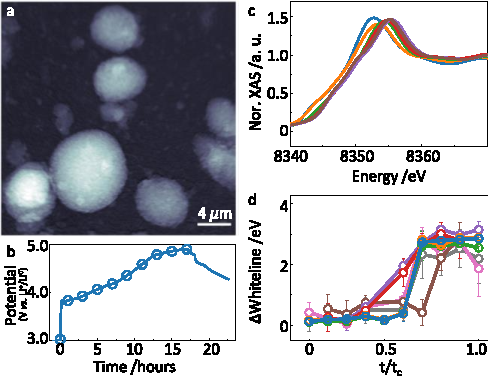
\includegraphics{figures/nca_txm.pdf}
  \caption{Operando \gls{txm} of \nca{} during first charge. (a) Mean
    optical depth frame of \nca{} particles. (b) Applied potential to
    operando cell during galvanostatic charging at \todo[inline]{what current,
      mA/g}. (c) Normalized spectra from \emph{ex-situ}
    ensemble-average \gls{xas}. (d) State-of-charge determined by
    whiteline position relative to overall state of charge in (c) for
    individual particles of \nca{}. Error bars represent one standard
    deviation over pixels within the given particle.}
  \label{fig:txm-nca}
\end{figure}

\begin{figure}
  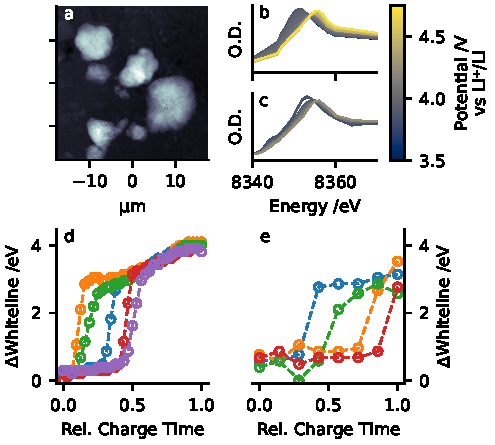
\includegraphics{figures/nmc_txm.pdf}
  \caption{Operando \gls{txm} \gls{xas} of \nmc[333]{} and \nmc[532]{}
    during first charge. (a) Mean optical depth frame of \nmc[333]{}
    particles. (b,c) Median optical depth spectra of active material
    during (b) second charge of \nmc[333]{} and (c) first charge of
    \nmc[532]{}. (d,e) Changes in median whiteline energies during
    first charge relative to start of charging for individual
    particles of (d) \nmc[333]{} (e) \nmc[532]{}.}
  \label{fig:txm-nmc}
\end{figure}

\begin{figure}
  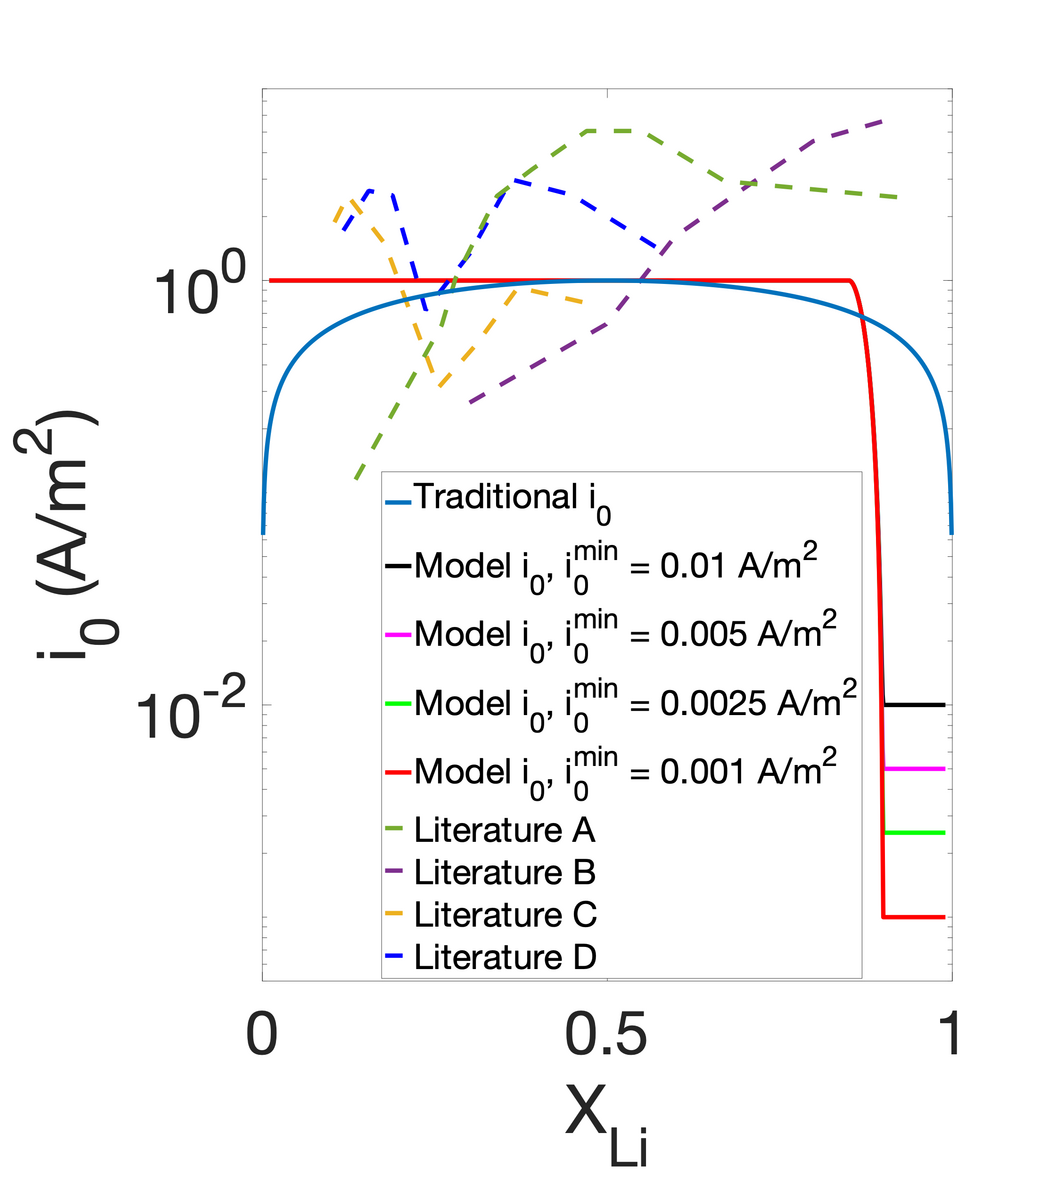
\includegraphics{figures/i0_profiles.png}
  \caption{Log scale comparison of different $i_0$ functions used in
    the sensitivity analyses. The literature-reported functions are
    shown in dashed lines. Plots labeled with Literature A and B are
    obtained from Ref.\ 9, Ref.xx, respectively, whereas plots labeled
    with Literature C and D are obtained from Ref.\ 8.}
  \label{fig:i0_profiles}
\end{figure}

\begin{figure}
  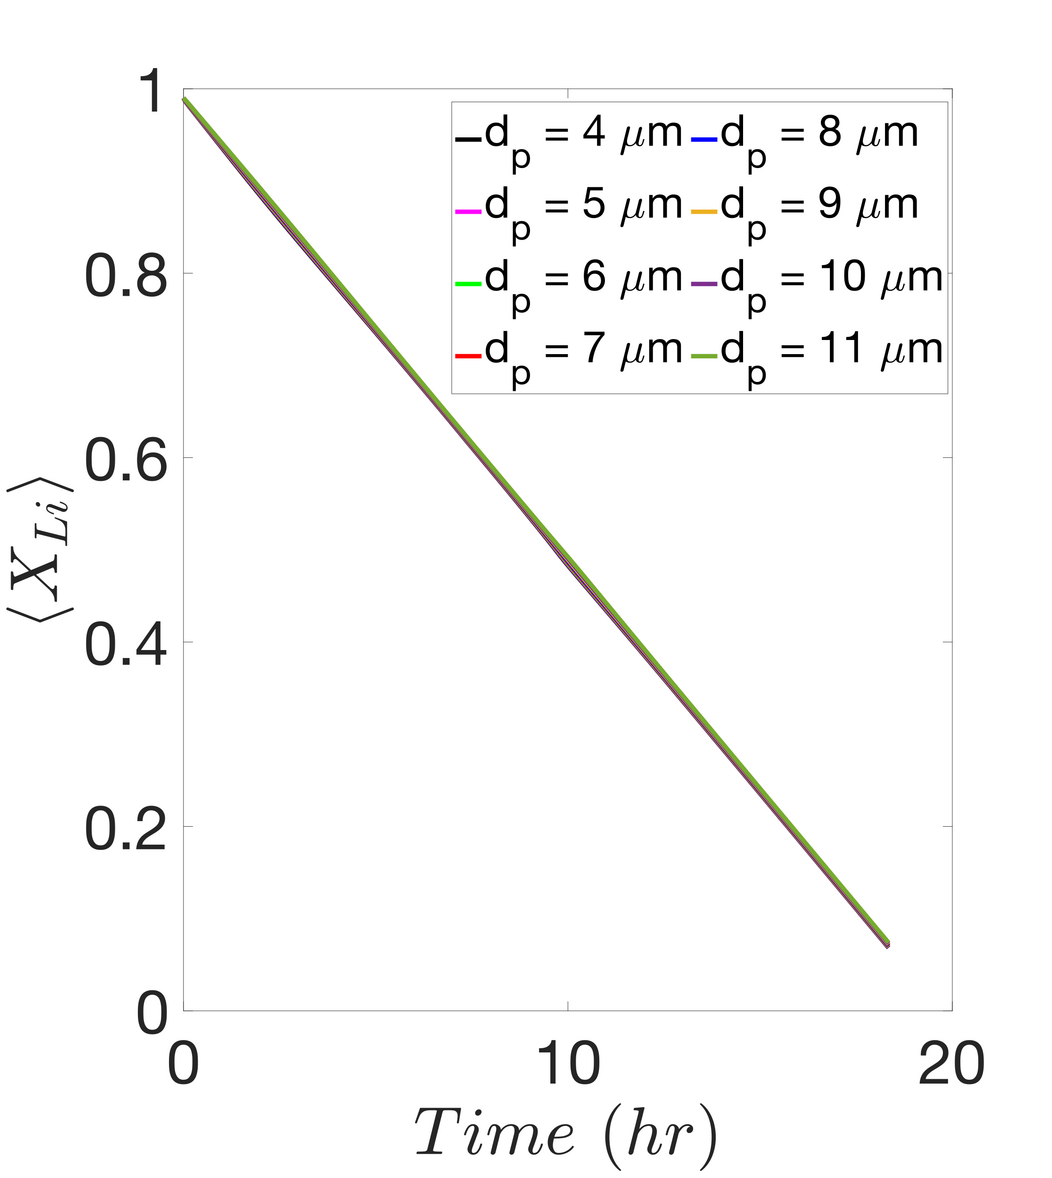
\includegraphics{figures/i0_basic.png}
  \caption{Evolution of $\left<X_{\rm{Li}}\right>$ for the 8-particle
    system obtained using the tradition function of $i_0$. All the
    particles delithiate at the same rate.}
  \label{fig:i0_basic}
\end{figure}

\begin{figure}
  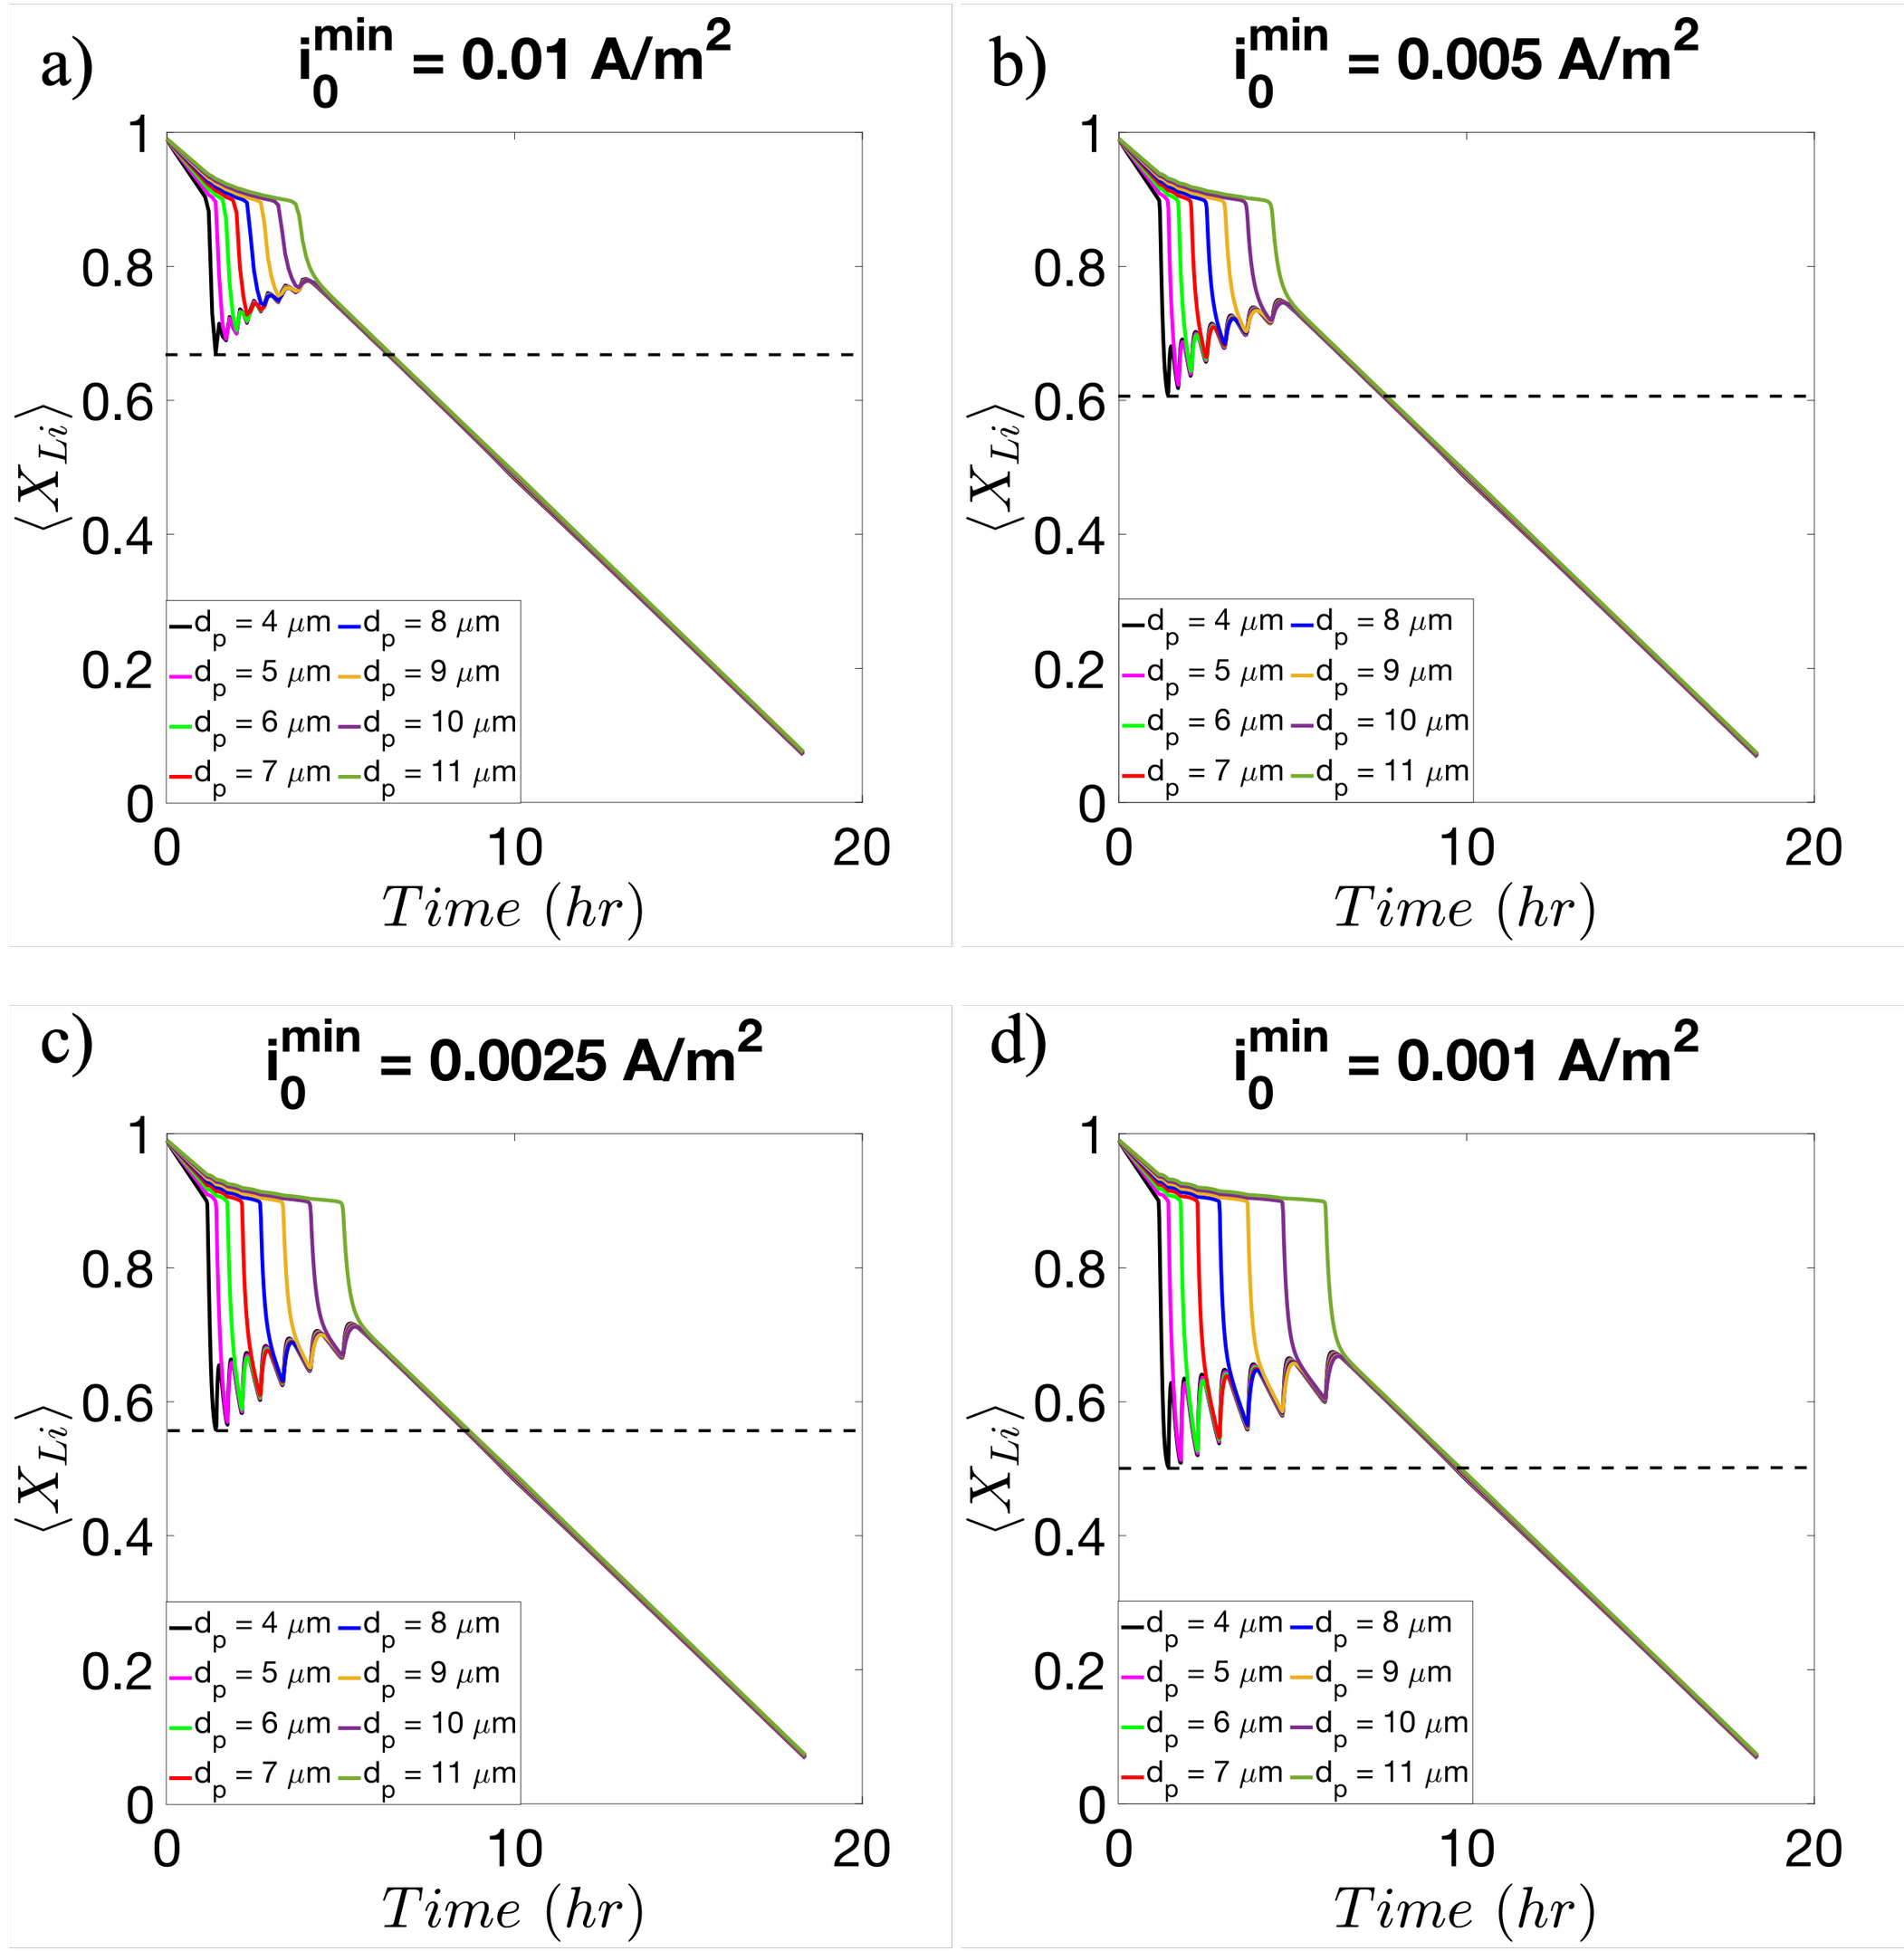
\includegraphics{figures/i0_models.png}
  \caption{Evolution of $\left<X_{\rm{Li}}\right>$ for the 8-particle
    system obtained using the model form of $i_0$ with four different
    values of $i_{0,\rm{min}}$: a)
    \SI{0.01}{\ampere\per\meter\squared}, b)
    \SI{0.005}{\ampere\per\meter\squared}, c)
    \SI{0.0025}{\ampere\per\meter\squared}, and d)
    \SI{0.001}{\ampere\per\meter\squared}. The black dashed line in
    each plot represents $\left<X_{\rm{Li}}\right>^\dagger$ for the
    smallest particle in the ensemble;
    $\left<X_{\rm{Li}}\right>^\dagger$ decreases with a decrease in
    $i_{0,\rm{min}}$.}
  \label{fig:i0_models}
\end{figure}

\begin{figure}
  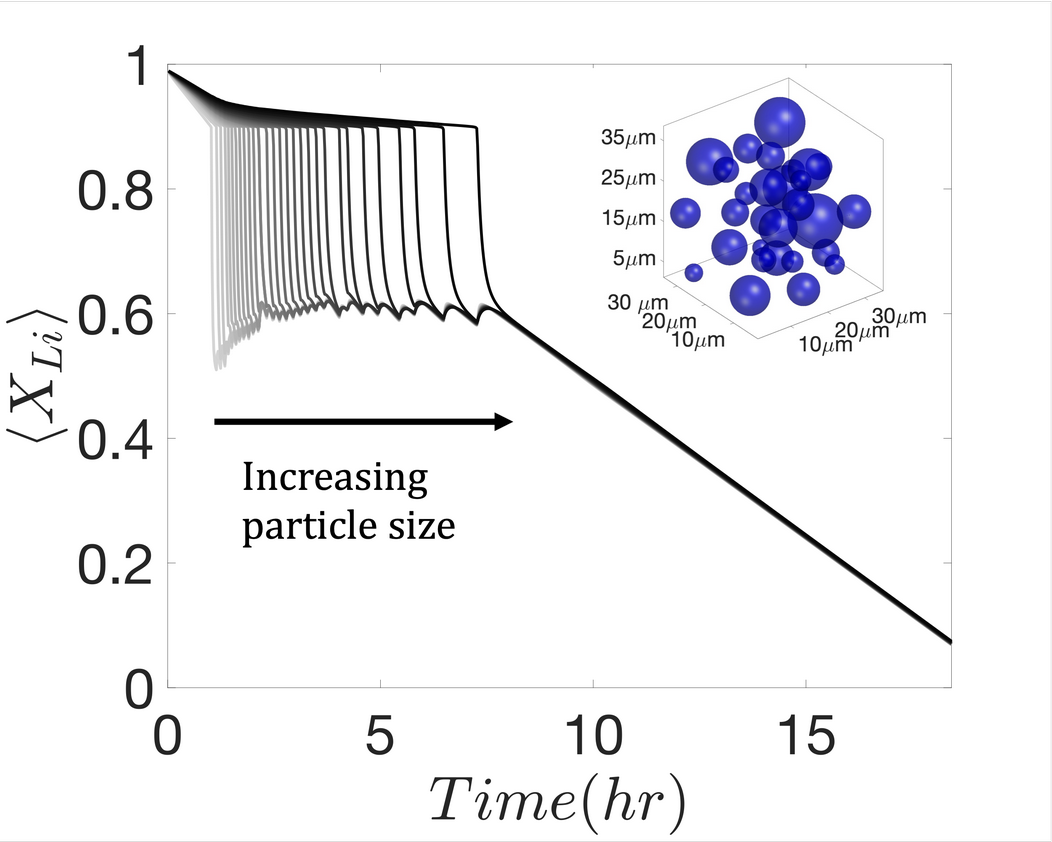
\includegraphics{figures/30_particles.png}
  \caption{Plot of $\left<X_{\rm{Li}}\right>$ vs.\ time for the
    30-particle system. The particles delithiate in the increasing
    order of their size. The inset shows the orientation of particles
    in the electrode.}
  \label{fig:30_particles}
\end{figure}

\begin{figure}
  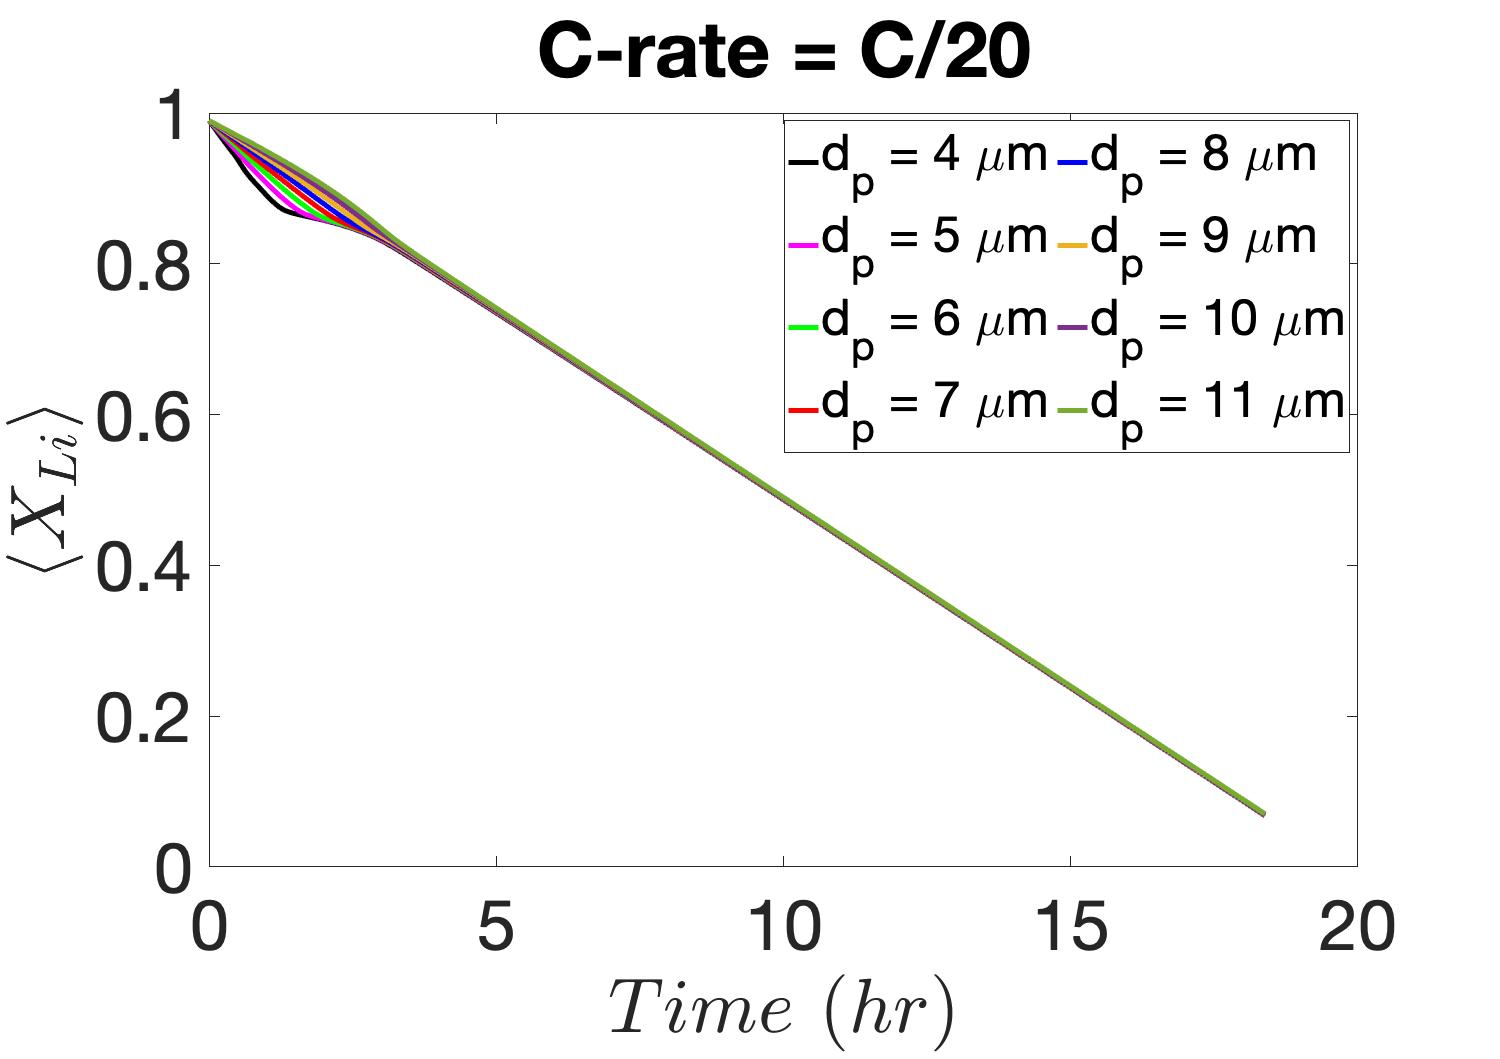
\includegraphics[width=\figwidth]{figures/Ds_profiles.jpg}
  \caption{}
  \label{fig:Ds_profiles}
\end{figure}

\begin{figure}
  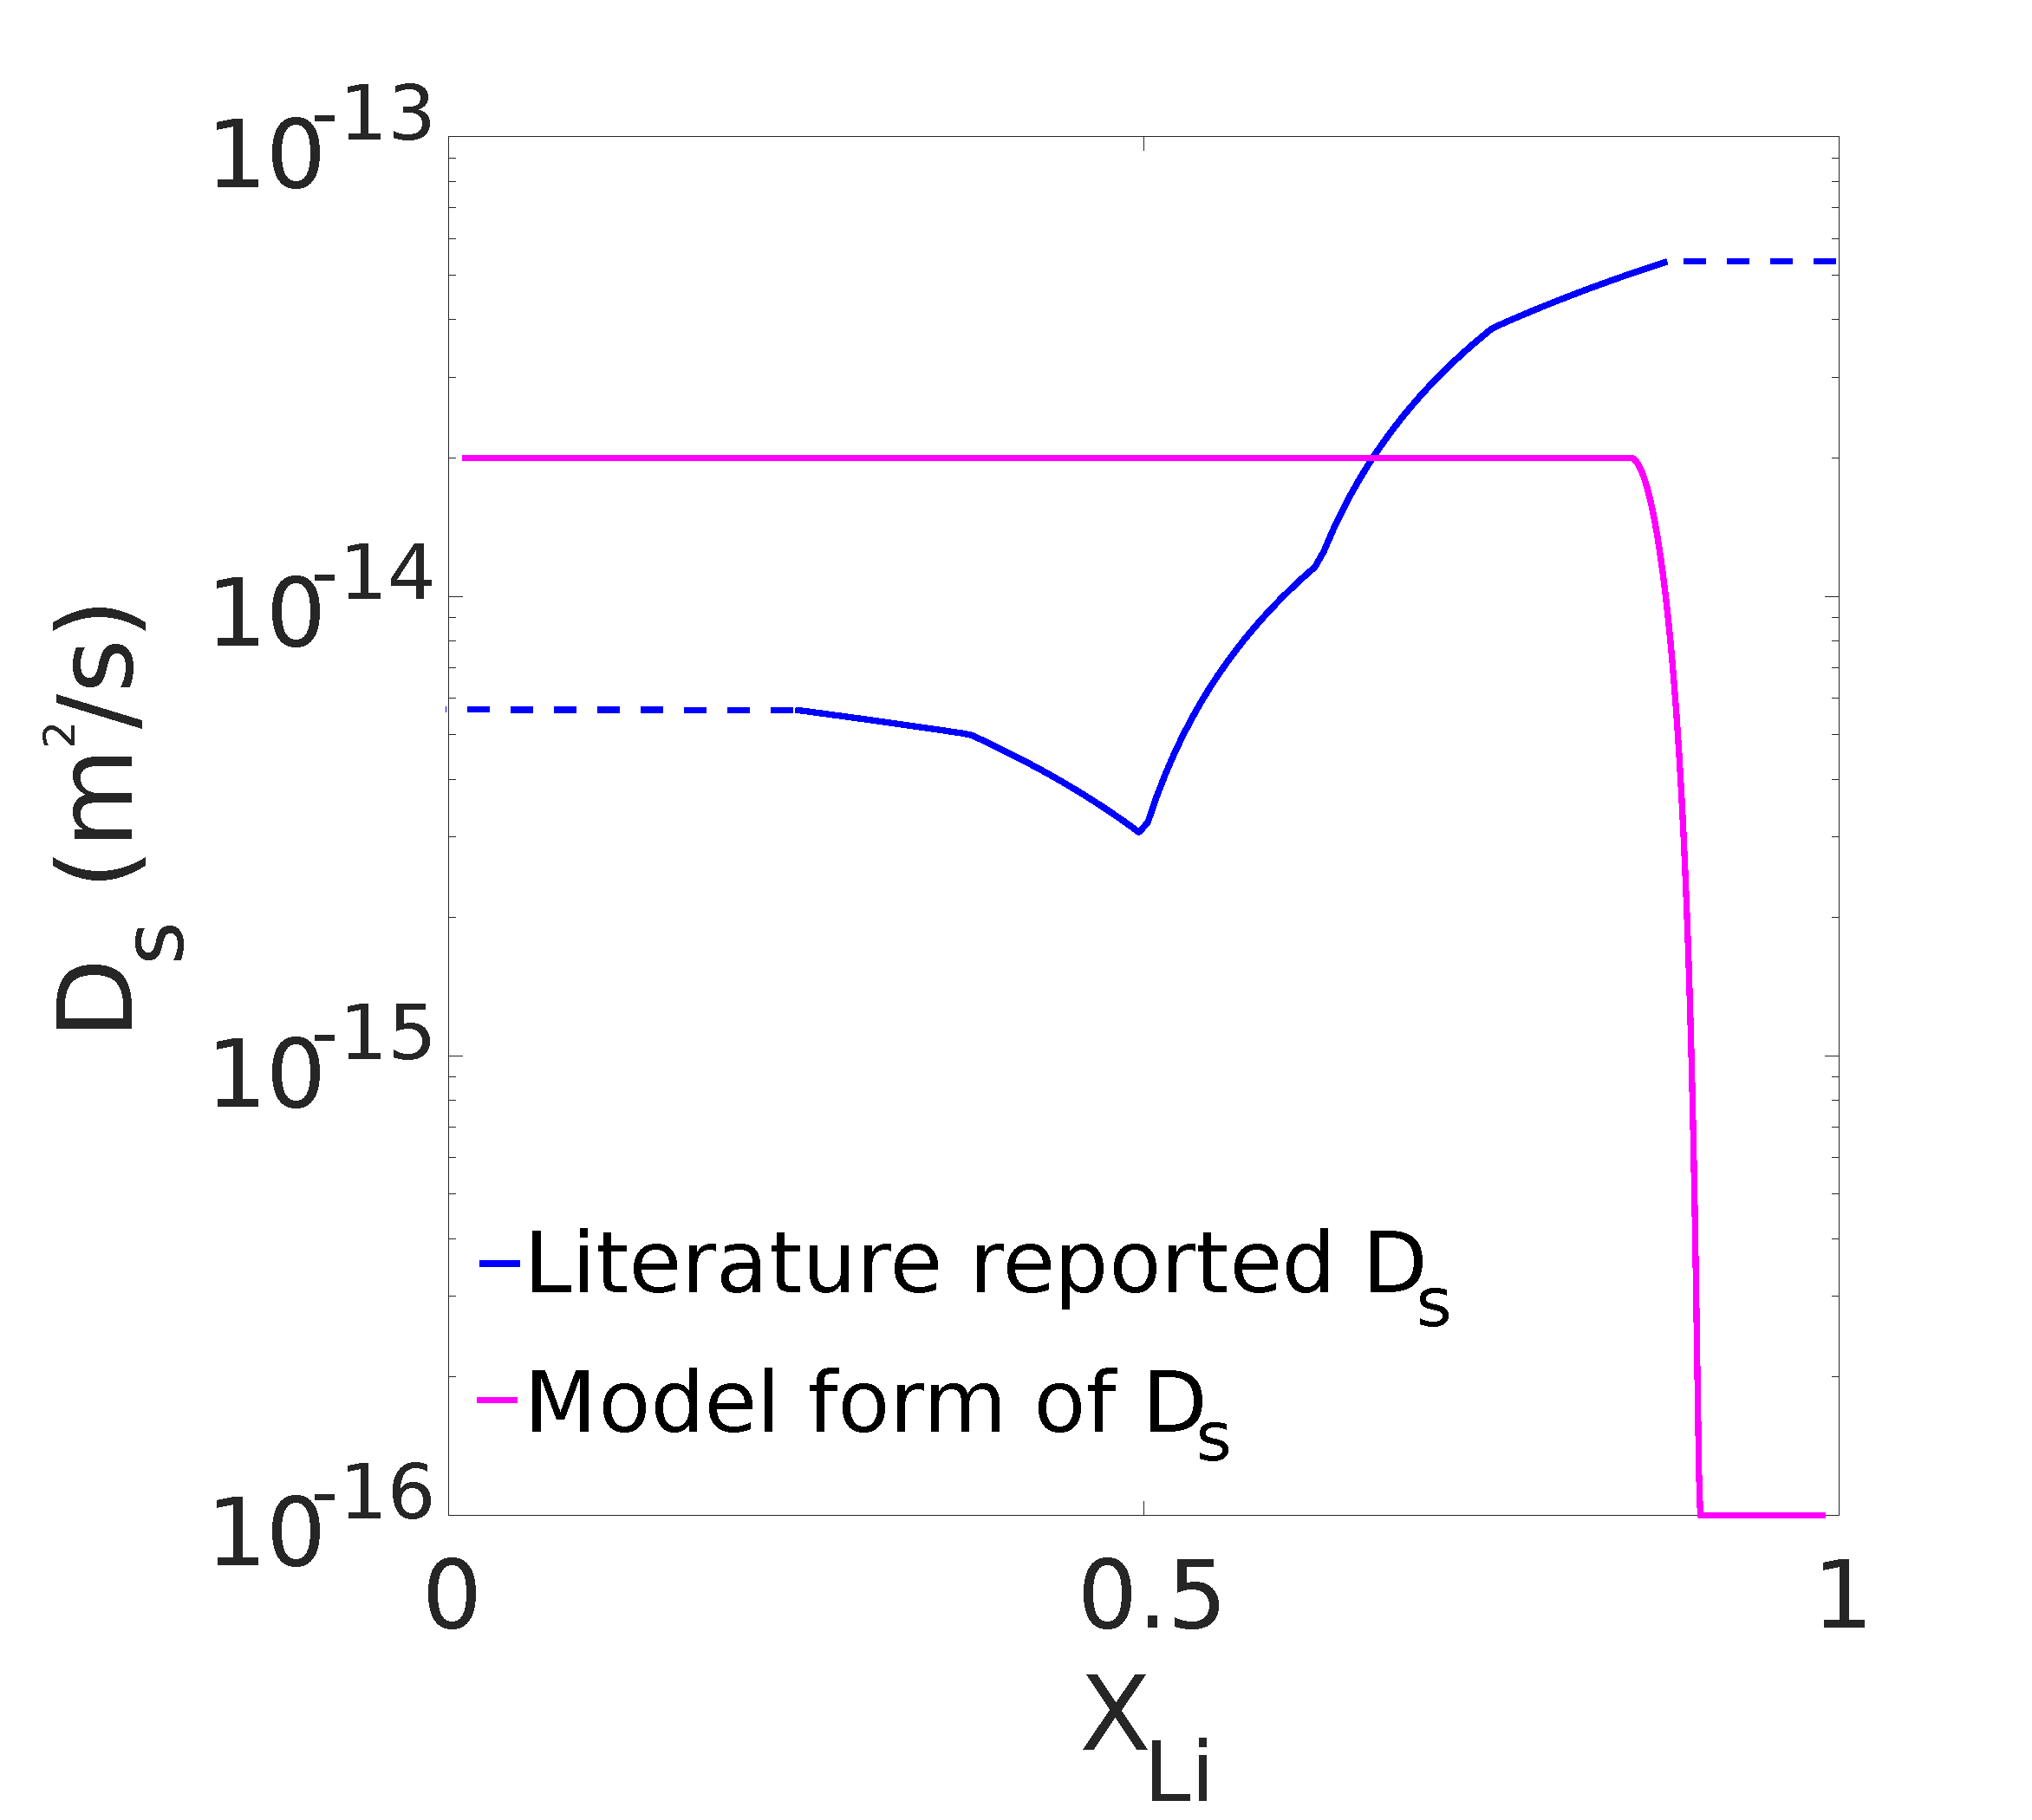
\includegraphics[width=\figwidth]{figures/Ds_comparison.pdf}
  \caption{Log scale comparison of the two $D_S$ functions used in the
    sensitivity analyses. The dashed lines for the literature reported
    function represent constant extrapolation used to determine the
    $D_S$ values beyond the range reported in the literature.}
  \label{fig:Ds_comparison}
\end{figure}


\bibliographystyle{plain}
\bibliography{refs,refs-extra}
%% \bibliography{references}

\end{document}
